% Source: graduate-coursework/Prior_Semesters/Fa23/CSCE350/assignments/HW2_Backward_Substitution.tex

\documentclass[border=4pt]{standalone}
\usepackage{amsmath}
\usepackage{tikz}
\usetikzlibrary{arrows}

\begin{document}
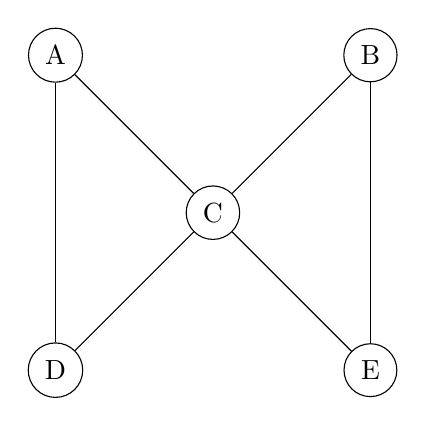
\begin{tikzpicture}[scale=2]
  \node[shape=circle,draw=black] (A) at (0,2) {A};
  \node[shape=circle,draw=black] (B) at (2,2) {B};
  \node[shape=circle,draw=black] (C) at (1,1) {C};
  \node[shape=circle,draw=black] (D) at (0,0) {D};
  \node[shape=circle,draw=black] (E) at (2,0) {E};
  \path [-] (A) edge node {} (C);
  \path [-] (B) edge node {} (C);
  \path [-] (D) edge node {} (C);
  \path [-] (E) edge node {} (C);
  \path [-] (A) edge node {} (D);
  \path [-] (B) edge node {} (E);
\end{tikzpicture}
\end{document}
